\section{Dataset Analysis}
\label{sec:analysis}

This section shows statistics of the \rover{} dataset and that users prefer aspect-specific, rooted facts.

\subsection{Dataset Statistics}
\label{sec:stats}
Table~\ref{tbl:stats} shows the basic statistics of the \rover{} dataset.
In total, our dataset contains \ndialogsfull{} dialogs with \nutterfull{} utterances.
The fact database contains \nfactsfull{} facts; of those, \nshownfull{} ($81\%$) were shown to the assistants and \nusedfull{} ($29\%$) were used in at least one message.
We randomly split dialogs into training, validation, and testing folds.

\begin{table}[t]
    \centering
    \scalebox{0.75}{
        \begin{tabular}{l r r r r r}
            \toprule
            \textbf{Metric (\# of)} & \textbf{Total}  & \textbf{Train}   & \textbf{Val}   & \textbf{Test}   & \textbf{Zero}       \\
            \midrule
            Dialogues               & \ndialogsfull{} & \ndialogstrain{} & \ndialogsval{} & \ndialogstest{} & \ndialogstestzero{} \\
            Utterances              & \nutterfull{}   & \nuttertrain{}   & \nutterval{}   & \nuttertest{}   & \nuttertestzero{}   \\
            Likes                   & \nlikedfull{}   & \nlikedtrain{}   & \nlikedval{}   & \nlikedtest{}   & \nlikedtestzero{}   \\
            Topics                  & \ntopicsfull{}  & \ntopicstrain{}  & \ntopicsval{}  & \ntopicstest{}  & \ntopicstestzero{}  \\
            Facts Total             & \nfactsfull{}   & NA               & NA             & NA              & NA                  \\
            Facts Shown             & \nshownfull{}   & \nshowntrain{}   & \nshownval{}   & \nshowntest{}   & \nshowntestzero{}   \\
            Facts Used              & \nusedfull{}    & \nusedtrain{}    & \nusedval{}    & \nusedtest{}    & \nusedtestzero{}    \\
            \bottomrule
        \end{tabular}
    }
    \caption{
        \rover{} has \ndialogsfull{} dialogs. On average, dialogs have $12.9$ utterances.
        $60\%$ of the assistants' 90,534 utterances were liked.
    }
    \label{tbl:stats}
\end{table}

\subsection{What Facts do User Prefer?}

In Section~\ref{sec:intro}, we hypothesized that when assistants use facts that mention previously known entities (rooted facts), users will be more likely to engage.
In our data collection, we incorporate two mechanisms to test this hypothesis.
The first mechanism is explicit: we directly ask users---through a like button---to indicate what messages they preferred.
The second mechanism is implicit and derived by mining dialogs for specific sequences of dialog acts that suggest engagement with the content.
For each of these mechanisms, we compute the likelihood $P(\text{Prefer}\g\text{Fact Source})$ of a user preferring utterances grounded to each fact source (Rooted, Aspect, or General).
Figure~\ref{fig:prefs} shows this likelihood and indicates that users prefer: (1) facts relevant to aspects versus general ones and (2) rooted facts in three of four scenarios.

\begin{figure}[t]
    \centering
    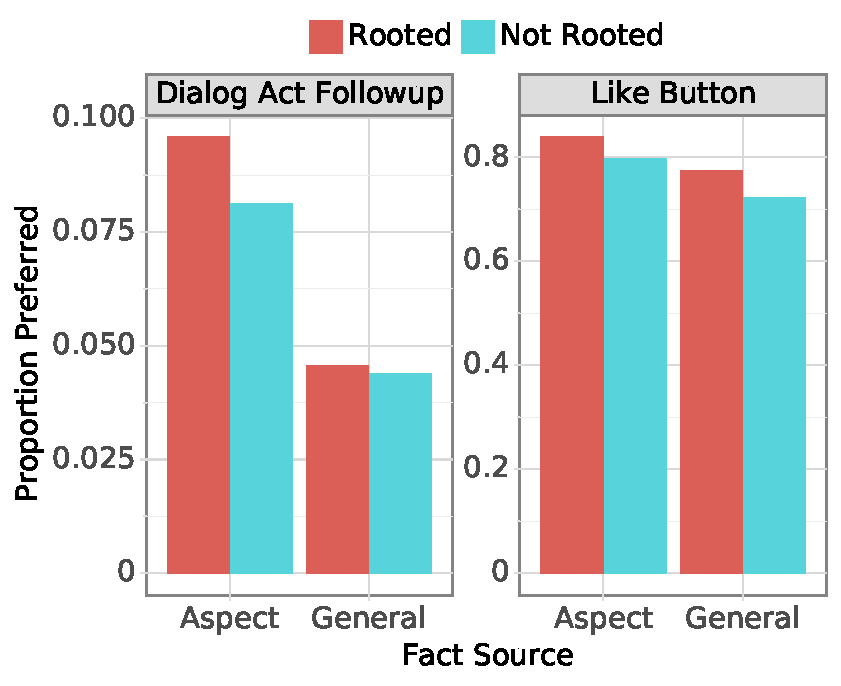
\includegraphics[width=\linewidth]{student_prefs}
    \caption{
        User engagement is measured by dialog act followups (left) and like button usage (right).
        We compare reactions to messages that use a fact mentioning an entity the user knew about (rooted) and whether the fact is general or aspect-specific.
        Pairwise differences are statistically significant ($99\%+$) with a two proportion z-test \emph{except} for dialog act followups between rooted and non-rooted general facts.
        Overall, users prefer on-aspect, rooted facts.
    }
    \vspace{-12pt}
    \label{fig:prefs}
\end{figure}

\subsubsection{Likes for Explicit Preference Elicitation}
Explicit preference is computed directly from like button usage and shown on the right panel of Figure~\ref{fig:prefs}.
Overall, users liked $60\%$ of messages, and they prefer on-aspect, rooted facts.

\subsubsection{Mining Acts for Implicit Preferences}
When users ask specific followup questions---as opposed to generic ones---about an assistant's fact, it shows that the user implicitly prefers these kinds of messages.
For example, asking about an entity like the Ta\'inos is more specific than asking about history and therefore indicates engagement.
We identify these interactions by mining for pairs of assistant-user messages where the assistant uses a fact and their message is labeled with an ``inform'' dialog act.
With these, we compute the likelihood
$$P(\text{Outcome}=\text{request\ followup}\g\text{Fact Source})$$
that the user's message has the ``request followup'' dialog act given the source.
Similarly to likes, users engage more with aspect-oriented and rooted facts.

\subsubsection{Paraphrase Analysis}
\label{sec:para-analysis}
Although our work does not include a paraphrase model, we manually analyze a random sample of two hundred and fifty assistant messages where facts were used. % where annotators indicated they used a fact
Of these messages, $51\%$ were acceptable paraphrases, $27\%$ were verbatim copies, $12\%$ were contextualizations of near copies, and the remainder were errors such as incorrect paraphrases or did not incorporate the fact.
Appendix~\ref{apx:para} shows descriptions, counts, and random examples of each category.
This analysis estimates that about half of grounded messages have non-trivial signal for future paraphrase models to use.
